 \documentclass[14pt]{beamer}
\usepackage[T1]{fontenc} 
\usepackage[utf8]{inputenc}
\usepackage[french]{babel}

\setbeamertemplate{blocks}[rounded]%[shadow=true]

%\usetheme[hideallsubsections]{Marburg}
\usetheme{CambridgeUS}

\title{\og Evaluating CRDTs for Real-time Document Editing \fg}
\subtitle{Summary}
\author{Ronan-Alexandre Cherrueau\\Adrien Bougouin\\Alban Ménager}

%		\begin{figure}
%			\includegraphics[scale=0.5]{includes/logoLina}
%			\label{fig:logoLina}
%   	\end{figure}

\begin{document}

\begin{frame}
	\titlepage
\end{frame}

\section*{Plan}
\begin{frame}
	\frametitle{Plan}
	\tableofcontents[hideallsubsections]
\end{frame}

\section{Introduction}
	\begin{frame}
		\frametitle{Introduction}
   		\begin{itemize}
    		\item Increasing of collaboring work and \emph{real-time}	 editing systems
    		\item A good example: Google Docs
    		\begin{itemize}
    			\item Allows editing on the same document at the same time by multiple authors.
    		\end{itemize}
    	\end{itemize}
	\end{frame}

\section{Existing}
	\begin{frame}
		\frametitle{Replication mechanism}
		\begin{itemize}
    		\item Real-time editing systems use replication mechanism to ensure consistency.
    		\item Optimistic replication gives to users a low time of latency.
		\end{itemize}
		\begin{figure}
			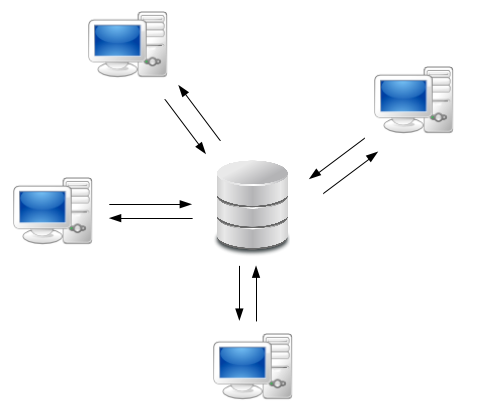
\includegraphics[scale=0.3]{includes/replication.png}
	   	\end{figure}
	\end{frame}
	\begin{frame}
		\frametitle{Problems}
		Centralized approach may cause problems:
		\begin{itemize}
			\item Personal datas are stored during the edition.
			\item It may be a privacy threat if they are used by corporations.
		\end{itemize}
	\end{frame}
	\begin{frame}
		\frametitle{Solution}
		\begin{itemize}
			\item Use decentralized mechanisms: Peer-to-peer.
			\item The main factor for suitable solutions is to respond to the users' actions in a reasonable time (about 50ms). 
		\end{itemize}
		\begin{figure}
			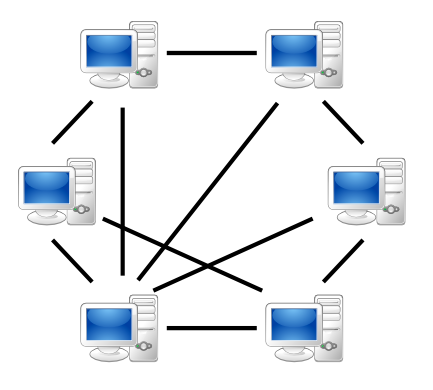
\includegraphics[scale=0.3]{includes/p2p.png}
	   	\end{figure}
	\end{frame}
	
\section{Goal of the experiment}
	\begin{frame}
		\frametitle{Goal}
		\begin{itemize}
			\item Select algorithms based on optimistic replication.
			\item Evaluate them on a decentralized real-time collaborative editing system.
			\item Evaluations based on real context on the same conditions and using the same data flow.
		\end{itemize}
	\end{frame}
	
\section{Approaches}
	\begin{frame}
		\frametitle{First approach: Operation transformation}
		\begin{itemize}
			\item Locally executed.
			\item Sent to others sites.
			\item Received by the centralized site.
			\item Transformed according to concurrent operations
			\item Executed on local copy.	
		\end{itemize}
	\end{frame}
	\begin{frame}
		\frametitle{New approach: CRDT}
		Commutative Replicated Data Types (CRDT)
		\begin{itemize}
			\item New class of replication mechanisms to preserve consistency.
			\item For peer-to-peer environment.
			\item The concurrent operations are natively commutative.
			\item The document is a linear sequence of elements.
			\item A single position identifier.
		\end{itemize}
	\end{frame}
	\begin{frame}
		\frametitle{Selected Algorithms}
		\begin{itemize}
			\item Logoot
			\item RGA
			\item WOOT
			\item WOOTO
			\item WOOTH
		\end{itemize}
	\end{frame}
	\begin{frame}
		\frametitle{Theoretical evaluation}
		\begin{figure}
			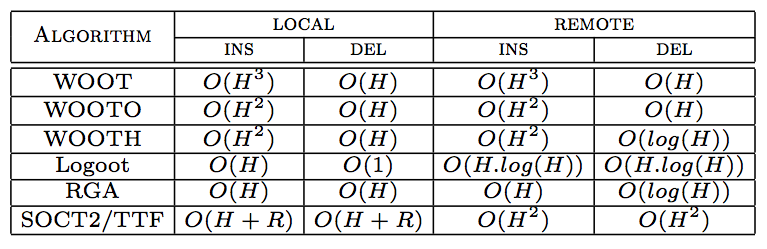
\includegraphics[scale=0.3]{../includes/worst.png}
			\caption{Worst-case time-complexity analysis}
	   	\end{figure}
	   	We see that RGA and Logoot have the bests results.
	\end{frame}
	
\section{Experiment}
	\begin{frame}
		\frametitle{Peer-to-Peer collaboration}
		\begin{itemize}
			\item The team designed a real-time peer-to-peer collaborations application.
			\item In order to obtain real logs.
			\item And apply logs to the algorithms.
		\end{itemize}
	\end{frame}
	\begin{frame}
		\frametitle{Groups for the experiments}
		\begin{itemize}
	\item 3 groups have to do their semester report by only using the collaborating editor for one hour and a half:
		\begin{itemize}
			\item 2 groups of 4 students.
			\item 1 group of 5 students.
		\end{itemize}
	\item 9 groups of 2 students have to translate an episode of \emph{The Big Bang Theory}
	\end{itemize}~
	1H30 for each experiment.
	\end{frame}
\section{Results}
	\begin{frame}
		\frametitle{Logs}
		\begin{figure}
  			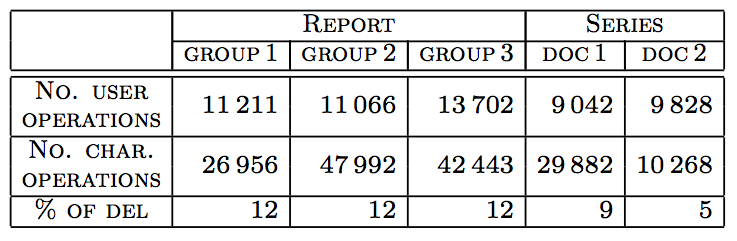
\includegraphics[width=0.7\textwidth]{../includes/operations.png}
  			\caption{Total number of user/character operations}
		\end{figure}
	\end{frame}
	\begin{frame}
		\frametitle{Users Operations: execution times - 2nd Group report}
		\begin{figure}
			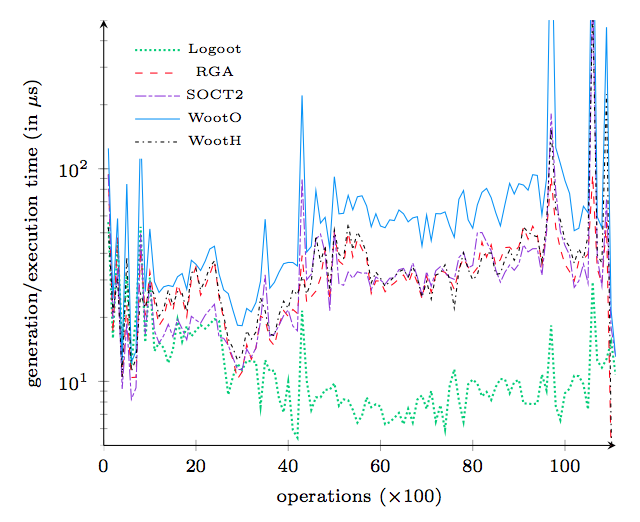
\includegraphics[width=.7\textwidth]{../includes/users_operations_2g_report.png}
		\end{figure}
	\end{frame}
	\begin{frame}
		\frametitle{Users Operations: execution times - 1st series}
		\begin{figure}
  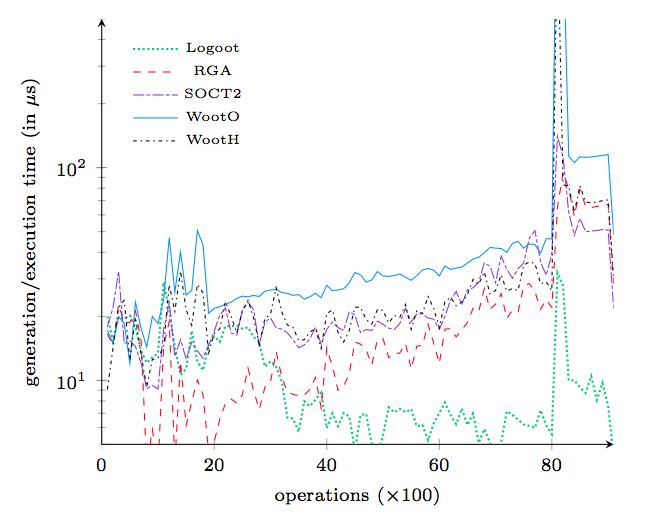
\includegraphics[width=.7\textwidth]{../includes/users_operations_1t_big.png}
		\end{figure}
	\end{frame}
	\begin{frame}
		\frametitle{Characters Operations: execution times - 2nd
group report}
		\begin{figure}
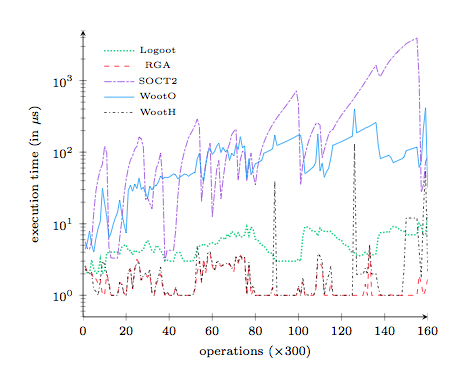
\includegraphics[width=.7\textwidth]{../includes/characters_operations_2g_report.png}
		\end{figure}
	\end{frame}
	\begin{frame}
		\frametitle{Characters Operations: execution times - 1 time
series}
		\begin{figure}
			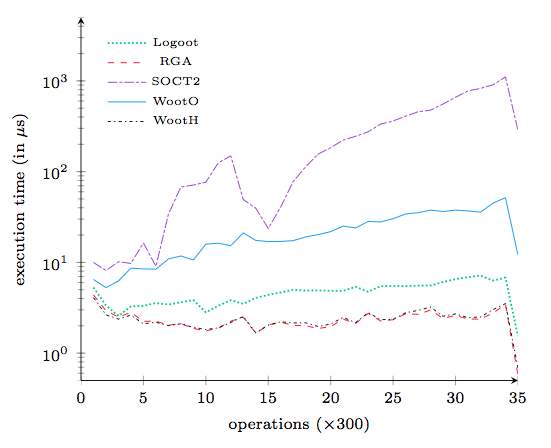
\includegraphics[width=.7\textwidth]{../includes/characters_operations_1t_big.png}
		\end{figure}
	\end{frame}
	
\section{Conclusion}
	\begin{frame}
		\frametitle{Conclusion}
		\begin{itemize}
			\item First performance evaluation of algorithms with real collaboration traces including concurrency.
			\item Proves the suitability of CRDT algorithms in real-time collaboration.
			\item Outperform some representative operational transformation approaches.
			\item Well established for real-time collaboration in terms of local generation time and remote integration time.
		\end{itemize}
	\end{frame}
\end{document}